\documentclass[10pt]{beamer}

\usepackage[utf8]{inputenc}
\usepackage{pgfpages}
\usepackage{dirtree}
%\setbeameroption{show notes on second screen =left} %hide nodes, show only notes, show notes on second screen = left.
\setbeamertemplate{note page}[plain]
\AtEndNote{\vfill \begin{center} mm:hh \end{center}}
\newcommand{\notedir}[1] {
  \note{\dirtree{#1}}}
\def \ion {$^{\circ}$ }
\usepackage{tcolorbox}
\usepackage{tikz}
\usetikzlibrary{intersections,calc}
\usepackage{amsmath}
\usepackage{graphicx}


\def \heart {\textcolor{blue}{$\heartsuit$} }
\def \C {$\mathcal{C}$}

\tcbset{%
	basic/.style={colframe=black,
		      colback=white,
		      top= 0mm,
		      bottom = 2mm,
		      boxsep=0mm
		      }
}

    
\begin{document}  
    \beamertemplatenavigationsymbolsempty
    
    \frame{%enoncé ex1
	  
	  \frametitle{Q1 Septembre 2015.}
	  On considère deux cercles $\mathcal{C}$ et $\mathcal{C'}$ se coupant en deux points distincts
	  $A$ et $B$. On note $P$ le point diamétralement opposé à $A$ sur $\mathcal{C}$, et $P'$ le
	  point diamétralement opposé à $A$ sur $\mathcal{C'}$ . \\
	  Démontrer que les points $P$ , $B$ et $P'$ sont alignés.
	  
	  \vfill
	  
	  \pause
	  % hypothèses et thèse
	  \begin{tcolorbox}[basic] 
	      \begin{columns}[t]
		 
		 \column{.5\textwidth}\centering
		      
		      \underline{Hypothèses} 
		      \begin{itemize}
		      \item $[AP]$ diamètre de $\mathcal{C}$ \\
			    $[AP']$ diamètre de  $\mathcal{C'}$,
		      \item $[AB]$ corde de $\mathcal{C}$ et $\mathcal{C'}$.			    
		      \end{itemize}

		  
		  \column{.5\textwidth}\centering
		      
		      \underline{Thèse} \\
		      \smallskip
		      $P,B$ et $P'$ alignés.
		
	      \end{columns}
	  \end{tcolorbox}
    \notedir{%
    .1 Énoncé.
    .2 Choix : Géométrie synthétique.
    .3 Présence de $\Delta$ et traduction analytique difficile..
    .4 Hypothèses (non visibles sur le dessin)..
    .4 Thèse..
    .4 Grand dessin.. 
    }
    }
    \frame{% résolution ex1

	  \begin{columns}[t]
		\column{.5\textwidth}\centering 
		

			\underline{Dessin}\\
			
				  \begin{figure}[h]
				  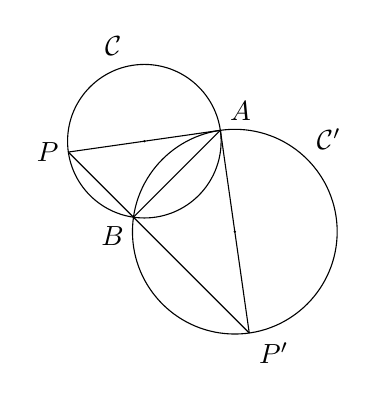
\begin{tikzpicture}[scale=0.65]
					%\draw[help lines] (-3,-3) grid (3,3); 					
					%CERCLE C
					\coordinate (O) at (0,0);
					\fill (O) circle (0.025);
					\draw[name path=cercle] (O) circle (1.5cm);
					\coordinate[label=above left:$\mathcal{C}$] () at (100:1.5);
					%CERCLE C'
					\coordinate (O') at (-45:2.5);
					\fill (O') circle (0.025);
					\draw[name path=cercle'] (O') circle (2cm);
					\path (O') -- +(45:2) coordinate[label=above right:$\mathcal{C'}$] ();

					
					%A et B
					\path [name intersections={of=cercle and cercle',by=intersection}];
					\coordinate[label=above right:$A$] (A) at (intersection-1);
					\coordinate[label=below left:$B$] (B) at (intersection-2);
					\draw (A) -- (O) -- +($(O)-(A)$) coordinate[label=left:$P$](P);
					\draw (A) -- (O') -- +($(O')-(A)$) coordinate[label=below right:$P'$](P');
					\draw (P) -- (P');
					\draw (A) -- (B);
					
				  \end{tikzpicture}
				  \end{figure}
			
				  \begin{tcolorbox}[basic] 
				      
				    \smallskip
				    \underline{Hypothèses} 
				    \begin{enumerate}
				    \item $[AP]$ diamètre de $\mathcal{C}$ \\
					  $[AP']$ diamètre de  $\mathcal{C'}$,
				    \item $[AB]$ corde de $\mathcal{C}$ et $\mathcal{C'}$.
				    \end{enumerate}
							      
				    \underline{Thèse} \\
				    \smallskip
				    $P,B$ et $P'$ alignés. 
				    \end{tcolorbox}
		
		
		\column{.5\textwidth}\centering
		
		\underline{Résolution}\\ \flushleft
		
		\heart Un triangle inscrit dans un demi-cercle est rectangle.
		
		
		\begin{enumerate}
		 \item $\Delta APB$ rectangle en $B$ \\
		       $\Delta AP'B$ rectangle en $B$,
		 \item $P$ et $P'$ sont sur une droite $\bot$ à AB passant par $B$.
		\end{enumerate}
		\bigskip		
		$P,B$ et $P'$ alignés.  \hfill $\qed$

   
	   \end{columns}
	 \notedir{%
	   .1 Prouver la thèse.
	   .2 Élément de théorie.
	   .3 Triangle inscrit dans demi-cercle..
	   .4 Implique des mesures d'angles..
	   .4 $PBP'$ sont alignés si $\widehat{PBP'}=180^{\circ}$..
	   .2 Résolution.
	   .3 Théorème des triangles inscrits dans demi-cercle..
	   .3 Application à $ABP$ et $ABP'$..
	   .4 $\widehat{ABP}=90^{\circ}$ et $\widehat{ABP'}=90^{\circ}$..
	   .5 $\widehat{PBP'}=180^{\circ} \rightarrow PBP'$ alignés..
	   }   
        }

  \frame{%énoncé ex2
	\frametitle{Q2 Septembre 2015.}
	 Dans un repère orthonormé $(O,X,Y)$, on considère une parabole $\mathcal{P}_1$
	 d’axe $Y$ dont le sommet est l’origine $O$ et dont tous les points ont
	 une ordonnée positive ou nulle. On considère aussi la parabole $\mathcal{P}_2$,
	 translatée de $\mathcal{P}_1$ , de sommet au point de coordonnées $(4, 0)$. Les
	 paraboles $\mathcal{P}_1$ et $\mathcal{P}_2$ sont telles que leurs tangentes respectives à leur
	 point d’intersection sont orthogonales. On demande de déterminer les
	 équations cartésiennes de $P_1$ et $P_2$.
  
	 \vfill
	  
	  \pause
	  % hypothèses et thèse
	  \begin{tcolorbox}[basic] \centering
	    
		      \smallskip
		      \underline{Procédé} \\ \smallskip
		      Équations de $\mathcal{P}_1, \mathcal{P}_2$ avec les conditions : \\ \medskip
		      \begin{columns}
		      \column{.30\textwidth}
		      
		      
		      $\mathcal{P}_1\begin{cases} 
				    \text{concavité positive,} \\
				    \text{sommet en }(0,0).
				    \end{cases}$
		      
		      \column{.30\textwidth}
		      $\mathcal{P}_2\begin{cases} 
				    \mathcal{P}_1 \text{ translatée,} \\
				    \text{sommet en }(4,0).
				    \end{cases}$
		     
		                     
		      \column{.30\textwidth}
		      Tangentes $\bot$ en $\mathcal{P}_1 \cap \mathcal{P}_2$.
		      \end{columns}
		      		      
	  \end{tcolorbox}
	  \notedir{%
	.1 Énoncé.
	.2 Choix : géométrie analytique.
	.3 Énoncé évoque un repère orthonormé..
	.4 Procédé : reformuler ce qu'il faut déterminer..
	.5 Caractéristiques des paraboles $\mathcal{P}_1$ et $\mathcal{P}_2$..
	}  
	}  
	
  \frame{ %résolution ex2
	\begin{columns}[t]
		\column{.5\textwidth}\centering 
		

			\underline{Dessin}\\
			
				  \begin{figure}[h]
				  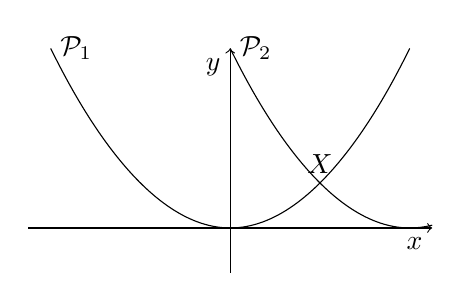
\begin{tikzpicture}[scale=0.57]
					%\draw[help lines] (-3,-3) grid (3,3); 				
					%AXES
					\draw[->] (0,-1) -- (0,4) coordinate[label=below left:$y$]();
					\draw[->] (-4.5,0) -- (4.5,0) coordinate[label=below left:$x$]();
					%P_1 et P_2
					\draw[name path = P_1] (-4,4) coordinate[label=right:$\mathcal{P}_1$]() parabola bend(0,0) (4,4);
					\draw[name path = P_2] (0,4) coordinate[label=right:$\mathcal{P}_2$]() parabola bend(4,0) (4.5,0.0625);
					\path [name intersections={of=P_1 and P_2,by=X}];
					\coordinate[label=above:$X$]() at (X); 
				  \end{tikzpicture}
				  \end{figure}
			
				  \begin{tcolorbox}[basic] 
				    \centering  
				    \smallskip
				    \underline{Procédé} \\ \smallskip
				    
				    Equations de $\mathcal{P}_1, \mathcal{P}_2$ avec les conditions : \\ \medskip				 
				    				    
				    $\mathcal{P}_1\begin{cases} 
						  \text{concavité positive,} \\
						  \text{sommet en }(0,0).
						  \end{cases}$ \\ \medskip

				    $\mathcal{P}_2\begin{cases} 
						  \mathcal{P}_1 \text{ translatée,} \\
						  \text{sommet en }(4,0).
						  \end{cases}$ \\ \smallskip

				    Tangentes $\bot$ en $\mathcal{P}_1 \cap \mathcal{P}_2$.

		      		      
				    \end{tcolorbox}
		
		
		\column{.5\textwidth}\flushleft
		
		\underline{Résolution}\\
		
		\begin{enumerate}

		\item[$\mathcal{P}_1$] $\equiv y=px^2$ $(p>0)$,
		\item[$\mathcal{P}_2$] $\equiv y=p(x-4)^2$,
		\item[$X$] $= \mathcal{P}_1 \cap \mathcal{P}_2 = (2,4p)$.
		\end{enumerate} \bigskip
		
		\heart Deux droites sont $\bot$ si le produit de leur coefficient angulaire vaut $-1$.
		 
	
		\begin{align*}
		\mathcal{P}_1'(2).\mathcal{P}_2'(2) =& -1& \\
		4p.-4p =& -1& \\
		p=& \text{ }\dfrac{1}{4} &\text{ car } p>0. \\ 
		\end{align*}
		
		$\begin{cases}\mathcal{P}_1\equiv y=\frac{x^2}{4} \\
			      \mathcal{P}_2\equiv y=\frac{(x-4)^2}{4}
		  \end{cases}$
		
		\hfill $\qed$
   
	   \end{columns}
  
	\notedir{%
	.1 Déterminer équations de $\mathcal{P}_1$ et $\mathcal{P}_2$.
	.2 Représenter les paraboles dans repère.
	.3 $\mathcal{P}_1$: equat\ion parabole avec concavité pos.~et sommet en O..
	.3 $\mathcal{P}_2$: $\mathcal{P}_1$ translatée de 4 vers x positifs..
	.3 $X$ point d'intersection des 2 paraboles..	
	.2 Résolution.
	.3 Tangentes $\bot$ en $X$.
	.4 Propriété des droites perpendiculaires.
	.5 Applications aux tangentes des paraboles en $X$.
	.6 Les pentes des tangentes sont données par les \\ \hspace{5mm} dérivées des paraboles en $X$..
	.7 On trouve $p$ et $p>0$ car $\mathcal{P}_1$ de concavité >0..
	.8 Équations de $\mathcal{P}_1$ et $\mathcal{P}_2$..
	}
	}
  
\end{document}
